\documentclass{beamer}
\usepackage[]{verbatim}
\usepackage{lmodern}
\usepackage{graphicx}
\usepackage[]{minted} 
\usepackage{tikz}
\usetikzlibrary{shapes.geometric, arrows, positioning, shadows}

\tikzstyle{container} = [draw, rectangle, minimum height=2cm, minimum width=3cm, text centered, text width=3cm, drop shadow, fill=blue!20, align=center]
\tikzstyle{component} = [draw, rectangle, minimum height=1cm, minimum width=2cm, text centered, text width=2cm, fill=green!10]
\tikzstyle{arrow} = [thick,->,>=stealth]

\title{Progress Report 1}
\subtitle{On the Data Input Tool for the SURGEAhead Intervention Study}
\author{U.~L.~Rieger}
\institute{Medical Systems Biology Group \\ Uni Ulm}
\date{\today} 

\begin{document}
\begin{frame}[t]
    \maketitle
\end{frame}

\begin{frame}[t]{Outline}
       \tableofcontents
\end{frame}

\section{Introduction}
\subsection{To SURGEAhead}%
\label{sub:To SU}

\begin{frame}{Introduction}
    \begin{block}{The SURGEAhead Project}
        \begin{itemize}
            \item Supporting SURgery with Geriatric Co-Managment and AI
            \item ``A study protocol for a digital geriatrician'' \cite{Leinert2023}
            \item Project aims to develop tools for \textit{post operative delirium} prediction 
            \item and a \textit{\textbf{c}ontinuity \textbf{o}f \textbf{c}are} tool (\textit{COC}).
            \item Where a first \textit{Observations- und KI-Entwicklungsstudie} (OKIE) study was conducted recently.
            \item OKIE studies data-input tool was a little patchy and required intense maintenance.
            \item Novel data-input tool is now implemented for the intervention study.
        \end{itemize}
    \end{block}
\end{frame}

\section{Current Software Layout}%
\label{sec:Current Software Layout}


\begin{frame}{Outline of the Data Input Tool}
\begin{figure}
\begin{center}
    \resizebox{\textwidth}{!}{
        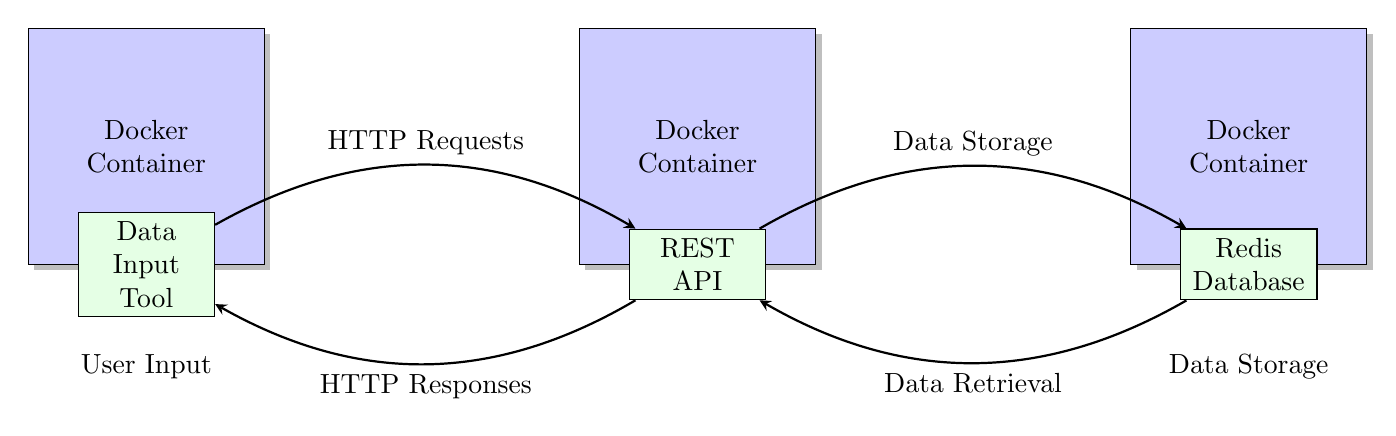
\begin{tikzpicture}[node distance=2cm]
            % Docker Containers
                  \node (DataInputToolContainer) [container, minimum height=3cm, minimum width=3cm, text width=2.5cm] {Docker Container};
                  \node (RestApiContainer) [container, right of=DataInputToolContainer, xshift=5cm, minimum height=3cm, minimum width=3cm, text width=2.5cm] {Docker Container};
                  \node (RedisContainer) [container, right of=RestApiContainer, xshift=5cm, minimum height=3cm, minimum width=3cm, text width=2.5cm] {Docker Container};

                  % Components inside Docker Containers
                  \node (DataInputTool) [component, below of=DataInputToolContainer, yshift=0.5cm, minimum height=0.75cm, minimum width=1.0cm, text width=1.5cm] {Data Input Tool};
                  \node (RestApi) [component, below of=RestApiContainer, yshift=0.5cm, minimum height=0.75cm, minimum width=1.5cm, text width=1.5cm] {REST API};
                  \node (Redis) [component, below of=RedisContainer, yshift=0.5cm, minimum height=0.75cm, minimum width=1.5cm, text width=1.5cm] {Redis Database};  % Arrows
            \draw [arrow, bend left] (DataInputTool) to node[midway, above] {HTTP Requests} (RestApi);
            \draw [arrow, bend left] (RestApi) to node[midway, above] {Data Storage} (Redis);
            \draw [arrow, bend left] (Redis) to node[midway, below] {Data Retrieval} (RestApi);
            \draw [arrow, bend left] (RestApi) to node[midway, below] {HTTP Responses} (DataInputTool);  % Labels
            \node [below of=DataInputTool, yshift=0.7cm] {User Input};
            \node [below of=RestApi, yshift=0.7cm] {};
            \node [below of=Redis, yshift=0.7cm] {Data Storage};
        \end{tikzpicture}
    }
\end{center}
\caption{A schematic representation of the data input tool. All components are running in separate Docker containers.}
\label{fig:1}
\end{figure}

\begin{block}{Advantages of using docker Containers}
    \begin{itemize}
        \item Isolation of components
        \item Security benefits
    \end{itemize}
    
\end{block}
\end{frame}

\section{Current Implementation}
\subsection{App}%
\label{sub:App}

\begin{frame}{Data Input Tool}
    \begin{block}{Data Input Tool}
        \begin{itemize}
            \item Implemented in Googles Flutter framework
            \item Based on the \textit{dart} programming language
            \item Supports different devices (mobile, web, and desktop) from a single codebase
        \end{itemize}
    \end{block}
    \begin{block}{On dart}
        Currently (2024-12-12) ranking place 33 ($0,47~\%$) in the \textit{TIOBE Index} \cite{TIOBE}, the language was developed by Google in 2011 as a modern option to javascript (JS ranks at place 6 with $4,61~\%$) in the TIOBE Index).
    \end{block}
\end{frame}

\begin{frame}[fragile]{Introduction to Dart}
    \begin{block}{Dart}
        \begin{itemize}
            \item Statically and strongly typed and `null` safe
            \item Object-oriented with classes and single inheritance
            \item Supports asynchronous programming
        \end{itemize}
    \end{block}
    \begin{minted}[
    frame=lines,
    framesep=2mm,
    fontsize=\footnotesize
    ]{dart}
void main() {
 int n = 10; // Number of terms in the Fibonacci series
 List<int> fibonacciSeries = List.generate(n, fibonacci);
 print(fibonacciSeries);
}

int fibonacci(int n) {
    if (n <= 1) {
        return n;
    } else {
        return fibonacci(n - 1) + fibonacci(n - 2);
    }
}
\end{minted}
\end{frame}

\begin{frame}[fragile]{Flutter}
    \begin{block}{Flutter}
        Dart-based SDK for building applications.
    \end{block}
    \begin{block}{Used by:}
        \begin{itemize}
            \item Google
            \item BMW
            \item Alibaba
            \item ByteDance
            \item Tencent
        \end{itemize}
    \end{block}

\end{frame}


%\begin{frame}[fragile]{Flutter}
%
%\begin{minted}[
%    frame=lines,
%    framesep=2mm,
%    fontsize=\footnotesize
%    ]{dart}
%import 'package:flutter/material.dart';
%void main() {
%  runApp(MyApp());
%}
%class MyApp extends StatelessWidget {
%  @override
%  Widget build(BuildContext context) {
%    return MaterialApp(
%      home: Scaffold(
%        appBar: AppBar(
%          title: Text('Hello, World!'),
%        ),
%        body: Center(
%          child: Text('Hello, World!'),
%        ),
%      ),
%    );
%  }
%}
%\end{minted}
%\end{frame} for  developed by Google.

\subsection{Database}%
\label{sub:Database}

\begin{frame}{Redis Database}
    \begin{block}{Redis}
        \begin{itemize}
            \item Fast in-memory data storage
            \item Key-value store
            \item Supports plenty data structures like:
                \begin{itemize}
                    \item strings
                    \item hashes
                    \item lists
                    \item and many more
                \end{itemize}
        \end{itemize}
    \end{block}
\end{frame}

\subsection{REST API}%

\begin{frame}{REST API}
        \begin{block}{REST API}
        \begin{itemize}
            \item Representational State Transfer
            \item Stateless
            \item Uses HTTP methods to perform CRUD operations (Create, Read, Update, Delete)
        \end{itemize}
    \end{block}
\begin{alertblock}{Note}
        Mainly needed as there is no Flutter package for direct communication with Redis application is compiled for web.
    \end{alertblock}

    \begin{block}{}
        In this project Pythons `flask` library is used to implement the REST API.
    \end{block}
\end{frame}
\begin{frame}{More on the input tool}
    \begin{block}{Basic functionalities}
        \begin{itemize}
            \item User authentication
            \item Assigning ID to new patients
            \item Write data associated with the patient to the database
            \item Read data from the database without the ability to modify it
        \end{itemize}
    \end{block}
\end{frame}

\section{Life demonstration}%
\label{sec:Life demonstration}

\begin{frame}{Life demonstration}
    \begin{block}{}
        \begin{itemize}
            \item Demonstration of the data input tool
        \end{itemize}
    \end{block}
\end{frame}

\section{Outlook}%
\label{sec:Outlook}
\begin{frame}{Outlook}
    \begin{block}{Next Steps}
        \begin{itemize}
            \item A status bar showing completeness of data for a patient
            \item Some kind of sorting mechanism for the assessments
            \item Add a proper authentication mechanism (e.g. Firebase)
            \item Implementation of real world assessments
        \end{itemize}
    \end{block}
\end{frame}

\begin{frame}{References} 
    \bibliography{biblio}
    \bibliographystyle{plain}
\end{frame}
\end{document}
